\documentclass[a4paper,11pt]{ltjsarticle}

\usepackage{amsmath}
\usepackage{amssymb}
\usepackage{bm}
\usepackage{mathtools}
\usepackage{graphicx}
\usepackage[hidelinks]{hyperref}
\usepackage{physics}
\usepackage{tikz}
\usetikzlibrary{
  arrows.meta,
  decorations.markings,
  patterns
}

\usepackage[section]{placeins}
\AddToHook{cmd/subsection/before}{\FloatBarrier}

% 二つの図で共通して使う設定
\tikzset{
  spacetime axis/.style={
    semithick,
    -{Stealth[length=2.3mm]}
  },
  spacetime path/.style={
    thick,
    postaction={decorate},
    decoration={
      markings,
      mark=at position 0.55 with {
        \arrow{Stealth[length=2.3mm]}
      }
    }
  },
  time slice/.style={
    draw=black!65,
    thin,
    pattern=north east lines,
    pattern color=black!18
  },
  event/.style={
    circle,
    fill=black,
    inner sep=1.6pt
  }
}
\newcommand{\qv}{\bm{q}}
\newcommand{\La}{\mathcal{L}}
\newcommand{\Laq}{\mathcal{L}(\qv(t),\dot{\qv}(t),t)}
\newcommand{\intS}{\int_{t_i}^{t_f}dt}
\newcommand{\ELeq}{\frac{d}{dt}\pdv{\Laq}{\dot{\qv}(t)}-\pdv{\Laq}{\qv(t)}}

\title{対称性と作用原理から力学を構成する
\\―Newton力学から特殊相対論へ―}
\author{本間海斗}
\date{}

\begin{document}

\maketitle

\begin{abstract}
本記事はLagrange形式から古典力学、特殊相対論を構築することを
目的とした。Lagrangianはよく天下り的に与えられ、既存の理論と整合するからという理由で
終わることがある。しかし、それではLagrange形式の真価が発揮されていないと私は思う。

この記事で主に次のことを意識した。\\
1.Newtonの運動方程式を前提とせず、それとは独立に古典力学を構築すること。
\\2.物理の本質部分からLagrangianを決定すること。
\\この2つを意識した。そのため、記事の構成としてはまず、古典力学の根本となる基礎
(前提)や定義、経験則を明確にし、その上で対称性というアプローチでLagrangianを決定した。
その際、できるだけ行間は埋め、論理をはっきりさせたつもりである。

記事の後半は特殊相対論をLagrange形式から構築する。
\end{abstract}

\tableofcontents

\section{古典力学の基礎}
この節では古典力学の基礎(前提)を書いた。以下の内容は
Lagrangianの決定で重要になる。


\subsection{基準系(定義)}

自然の中の様々な過程を記述するには基準系が必要である。ここに、基準系とは粒
子の空間的位置を指定する座標系と、時刻を指定するためのこの系に固定された時計
とを合わせたものである。

\FloatBarrier
\subsection{非相対論的時空(仮定)}
\label{sec:Spacetime}
非相対論的力学では、すべての基準系に共通する絶対時間が存在すると仮定する。したがって、
二つの事象の時間間隔は基準系によらない。また、同時刻における空間は3次元ユーク
リッド空間であり、同時刻に起きた二事象の空間距離は基準系によらないと仮定する。
\\数式で表すと、ある事象を基準系 $K$ では $(t,\bm{x})$ で表し、 $K^\prime$ では $(t^\prime , \bm{x}^\prime)$ とすると、
異なる時刻での事象の時間間隔は、
\[
\varDelta t=\varDelta t^\prime
\]
を満たし、同時刻での事象の空間的間隔は
\[
|\varDelta\bm{x}|=|\varDelta\bm{x}^\prime|
\]
が成り立つということである。(図\ref{fig:distance},\ref{fig:time})
\\この仮定はGalilei変換を導出するのに用いる。(\ref{sec:Hosoku})

\begin{figure}[htbp]
  \centering
  \begin{tikzpicture}[scale=0.85]

    % ---------- K系 ----------
    \begin{scope}
      \node at (1.0,3.65) {$K$};

      % 等時刻面
      \path[time slice]
        (-0.85,1.95) -- (2.65,1.95)
        -- (3.15,2.65) -- (-0.35,2.65)
        -- cycle;
      \node[right] at (3.15,2.30) {$t$};

      % 座標軸
      \draw[spacetime axis]
        (0,0) -- (-1.35,-1.25)
        node[below left] {$x$};
      \draw[spacetime axis]
        (0,0) -- (3.05,0)
        node[right] {$y$};
      \draw[spacetime axis]
        (0,0) -- (0,3.20)
        node[above] {$t$};

      % 世界線
      \draw[spacetime path]
        (0.30,-0.60)
        .. controls (0.60,0.05) and (0.00,1.10) ..
        (0.65,2.30);

      \draw[spacetime path]
        (1.85,-0.60) -- (1.85,2.30);

      % 同時刻の二点
      \node[event] (C) at (0.65,2.30) {};
      \node[event] (D) at (1.85,2.30) {};

      \node[left=5pt] at (C) {$C$};
      \node[right=5pt] at (D) {$D$};

      \node[above] at (0.65,2.73) {$\bm{x}_C(t)$};
      \node[above] at (2.05,2.73) {$\bm{x}_D(t)$};

      % 距離
      \node at (1.0,-1.95)
        {$|\Delta \bm{x}|=|\bm{x}_D(t)-\bm{x}_C(t)|$};
    \end{scope}

    % ---------- K'系 ----------
    \begin{scope}[shift={(7.2,0)}]
      \node at (1.0,3.65) {$K'$};

      % 等時刻面
      \path[time slice]
        (-0.85,1.95) -- (2.65,1.95)
        -- (3.15,2.65) -- (-0.35,2.65)
        -- cycle;
      \node[right] at (3.15,2.30) {$t'$};

      % 座標軸
      \draw[spacetime axis]
        (0,0) -- (-1.35,-1.25)
        node[below left] {$x'$};
      \draw[spacetime axis]
        (0,0) -- (3.05,0)
        node[right] {$y'$};
      \draw[spacetime axis]
        (0,0) -- (0,3.20)
        node[above] {$t'$};

      % 世界線
      \draw[spacetime path]
        (0.15,-0.60)
        .. controls (0.55,0.15) and (0.75,1.45) ..
        (1.30,2.30);

      \draw[spacetime path]
        (1.35,-0.60) -- (2.50,2.30);

      % 同時刻の二点
      \node[event] (Cp) at (1.30,2.30) {};
      \node[event] (Dp) at (2.50,2.30) {};

      \node[left=5pt] at (Cp) {$C'$};
      \node[right=3pt] at (Dp) {$D'$};

      \node[above] at (1.15,2.73) {$\bm{x}'_C(t')$};
      \node[above] at (2.65,2.73) {$\bm{x}'_D(t')$};

      % 距離
      \node at (1.0,-1.95)
        {$|\Delta \bm{x}'|=|\bm{x}'_D(t')-\bm{x}'_C(t')|$};
    \end{scope}

    % 共通の結論
    \node at (4.6,-2.85)
      {同時刻において
        $|\Delta \bm{x}|=|\Delta \bm{x}'|$};

  \end{tikzpicture}
  \caption{非相対論的時空：同時刻の二点間距離の不変性}
  \label{fig:distance}
\end{figure}

\begin{figure}[htbp]
  \centering
  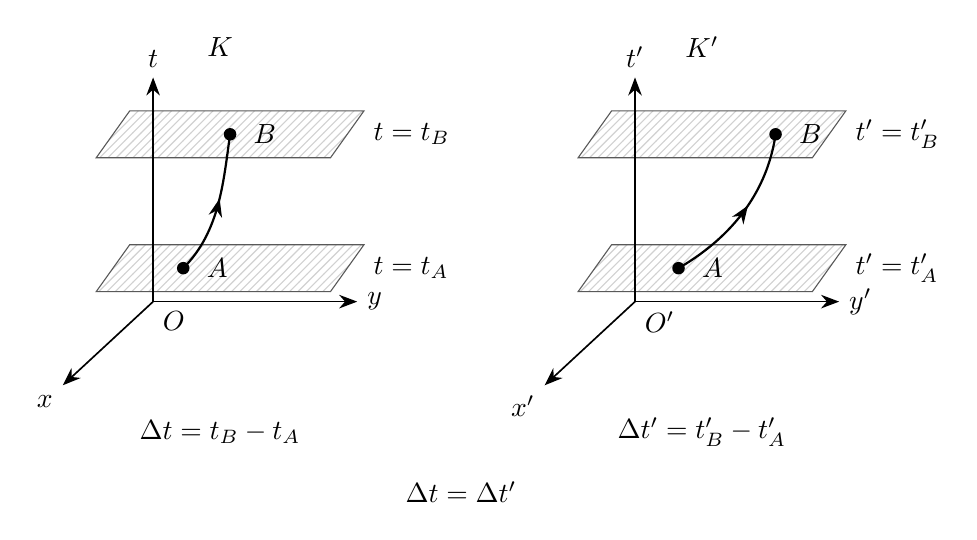
\begin{tikzpicture}[scale=0.85]

    % ---------- K系 ----------
    \begin{scope}
      \node at (1.0,3.80) {$K$};

      % 下の等時刻面
      \path[time slice]
        (-0.85,0.15) -- (2.65,0.15)
        -- (3.15,0.85) -- (-0.35,0.85)
        -- cycle;
      \node[right] at (3.15,0.50) {$t=t_A$};

      % 上の等時刻面
      \path[time slice]
        (-0.85,2.15) -- (2.65,2.15)
        -- (3.15,2.85) -- (-0.35,2.85)
        -- cycle;
      \node[right] at (3.15,2.50) {$t=t_B$};

      % 座標軸
      \draw[spacetime axis]
        (0,0) -- (-1.35,-1.25)
        node[below left] {$x$};
      \draw[spacetime axis]
        (0,0) -- (3.05,0)
        node[right] {$y$};
      \draw[spacetime axis]
        (0,0) -- (0,3.35)
        node[above] {$t$};
      \node[below right] at (0,0) {$O$};

      % AからBへの世界線
      \draw[spacetime path]
        (0.45,0.50)
        .. controls (1.00,1.05) and (1.05,1.80) ..
        (1.15,2.50);

      \node[event] (A) at (0.45,0.50) {};
      \node[event] (B) at (1.15,2.50) {};

      \node[right=5pt] at (A) {$A$};
      \node[right=5pt] at (B) {$B$};

      % 時間間隔
      \node at (1.0,-1.95)
        {$\Delta t=t_B-t_A$};
    \end{scope}

    % ---------- K'系 ----------
    \begin{scope}[shift={(7.2,0)}]
      \node at (1.0,3.80) {$K'$};

      % 下の等時刻面
      \path[time slice]
        (-0.85,0.15) -- (2.65,0.15)
        -- (3.15,0.85) -- (-0.35,0.85)
        -- cycle;
      \node[right] at (3.15,0.50) {$t'=t'_A$};

      % 上の等時刻面
      \path[time slice]
        (-0.85,2.15) -- (2.65,2.15)
        -- (3.15,2.85) -- (-0.35,2.85)
        -- cycle;
      \node[right] at (3.15,2.50) {$t'=t'_B$};

      % 座標軸
      \draw[spacetime axis]
        (0,0) -- (-1.35,-1.25)
        node[below left] {$x'$};
      \draw[spacetime axis]
        (0,0) -- (3.05,0)
        node[right] {$y'$};
      \draw[spacetime axis]
        (0,0) -- (0,3.35)
        node[above] {$t'$};
      \node[below right] at (0,0) {$O'$};

      % AからBへの世界線
      \draw[spacetime path]
        (0.65,0.50)
        .. controls (1.60,1.05) and (2.00,1.80) ..
        (2.10,2.50);

      \node[event] (Ap) at (0.65,0.50) {};
      \node[event] (Bp) at (2.10,2.50) {};

      \node[right=5pt] at (Ap) {$A$};
      \node[right=5pt] at (Bp) {$B$};

      % 時間間隔
      \node at (1.0,-1.95)
        {$\Delta t'=t'_B-t'_A$};
    \end{scope}

    % 共通の結論
    \node at (4.6,-2.85)
      {$\Delta t=\Delta t'$};

  \end{tikzpicture}
  \caption{非相対論的時空：時間間隔の不変性}
  \label{fig:time}
\end{figure}

\FloatBarrier
\subsection{運動の決定性(経験則)}
\label{sec:Motion}
3次元空間において拘束のない $N$ 個の粒子系の力学的自由度は $3N$ である。粒子の位置を記述
するために$3N$次元配位空間上で一般化座標 
\[
\bm{q}(t)=\bigl(q_1(t),q_2(t),\ldots,q_{3N}(t)\bigr)
\]
を定義し、一般化速度をその導関数として 
\[
\dot{\bm{q}}(t)=\bigl(\dot{q}_1(t),\dot{q}_2(t),\ldots,\dot{q}_{3N}(t)\bigr)
\]
と定義する。

古典粒子力学では、ある時刻に \(\bm{q},\dot{\qv}\) を指定すると、
その直後の時間発展が一意に定まることを経験則として仮定する。
このことはすなわち、粒子の(一般化)加速度が位置と速度の関数で一意的に表せることを意味する。
\begin{equation}
\ddot{\bm{q}}(t)=\bm{f}\bigl(\bm{q}(t),\dot{\bm{q}}(t),t\bigr)
\label{eq:accelaration}
\end{equation}
これにより、ある時刻での全粒子の位置と速度が与えられれば、その時刻 $t$ での全粒子の(一般化)加速度が(\refeq{eq:accelaration})により定まり、そこから微小時間 $dt$
だけ経過した時刻での位置と速度は
\begin{align*}
\dot{\qv}(t+dt)&\simeq\dot{\qv}(t)+\ddot{\qv}(t)dt\\
\qv(t+dt)&\simeq\qv(t)+\dot{\qv}(t)dt
\end{align*}
で求めることができる。(ここで、$(dt)^2$ 以上は無視した) そして、(\refeq{eq:accelaration})式により、時刻 $t+dt$ での加速度が定まるため、
さらに $dt$ だけ経過した時も同様に計算できる。
一般に、(\refeq{eq:accelaration})式を運動方程式と言う。
次の節で運動方程式(\refeq{eq:accelaration})を与える方法(原理)を示す。

\section{停留作用の原理}

\subsection{Lagrangianと作用}
粒子の運動は停留作用の原理から与えられ、おのおのの系はLagrangianと呼ばれる関数 $\La$ で記述される。
\ref{sec:Motion} 節より、運動方程式は 2 階の微分方程式である。そのため、古典力学の運動方程式を高々2階に保つためLagrangian $\La$ は
$\qv(t)$ , $\dot{\qv}(t)$ , $t$ の関数であると仮定する。
\\作用 $S$ は粒子の軌道 $\qv(\cdot)$ を引数とする汎関数として次のように記述される。
\[
S[\qv(\cdot)]:=\int_{t_i}^{t_f}dt\Laq
\]
作用は粒子の軌道 $\qv(\cdot)$ を一つ定めると値が決まるという関係にある。(図\ref{fig:Mapping})
\[
\qv(\cdot) \longmapsto S[\qv(\cdot)]
\]
ここで、作用の引数が$\bm{q}(\cdot)$となっているのは、$\bm{q}(\cdot)$は関数形であり、これと実数である$q_i(t)$とを区別するためである。

\begin{figure}[htbp]
  \centering
  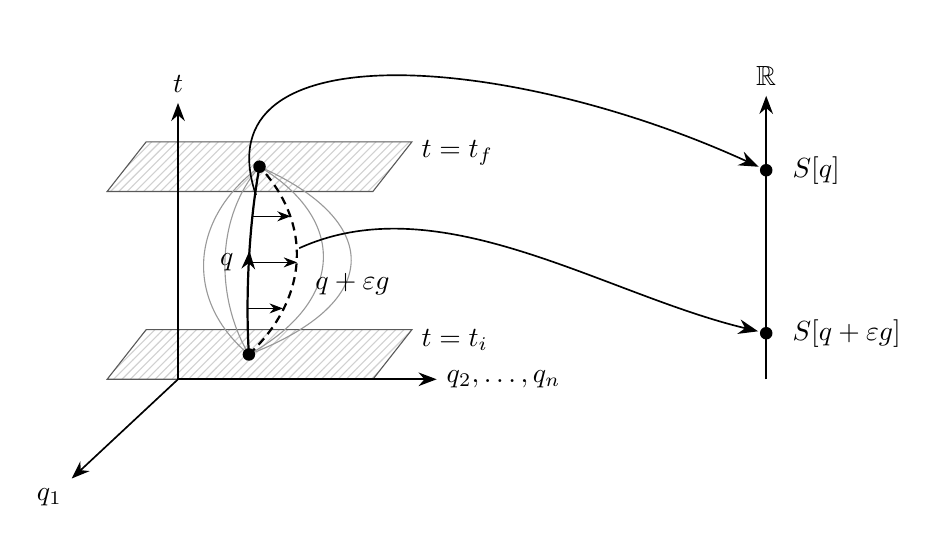
\begin{tikzpicture}[scale=0.9]

    % ---------- 等時刻面 ----------
    % t = t_i
    \path[time slice]
      (-1.00,0.00) -- (2.75,0.00)
      -- (3.30,0.70) -- (-0.45,0.70)
      -- cycle;
    \node[right] at (3.30,0.55) {$t=t_i$};

    % t = t_f
    \path[time slice]
      (-1.00,2.65) -- (2.75,2.65)
      -- (3.30,3.35) -- (-0.45,3.35)
      -- cycle;
    \node[right] at (3.30,3.20) {$t=t_f$};

    % ---------- 座標軸 ----------
    \draw[spacetime axis]
      (0,0) -- (-1.50,-1.40)
      node[below left] {$q_1$};

    \draw[spacetime axis]
      (0,0) -- (3.65,0)
      node[right] {$q_2,\ldots,q_n$};

    \draw[spacetime axis]
      (0,0) -- (0,3.90)
      node[above] {$t$};

    % ---------- 共通の端点 ----------
    \coordinate (I) at (1.00,0.35);
    \coordinate (F) at (1.15,3.00);

        % ---------- その他の候補経路 ----------
    % すべて同じ端点 I, F を通る

    % 左側へ膨らむ経路
    \draw[thin,black!40]
      (I)
      .. controls (0.10,1.10) and (0.15,2.25) ..
      (F);

    \draw[thin,black!40]
      (I)
      .. controls (0.55,1.10) and (0.50,2.25) ..
      (F);

    % 右側へ膨らむ経路
    \draw[thin,black!40]
      (I)
      .. controls (2.35,1.10) and (2.40,2.25) ..
      (F);

    \draw[thin,black!40]
      (I)
      .. controls (2.95,1.10) and (2.85,2.25) ..
      (F);
    % 元の経路 q
    \draw[spacetime path]
      (I)
      .. controls (0.95,1.15) and (1.00,2.20) ..
      (F);

    % 変分した経路 q + epsilon g
    \draw[thick,densely dashed]
      (I)
      .. controls (1.85,1.15) and (1.90,2.20) ..
      (F);

    % 変分を示す横向きの矢印
    \foreach \xa/\xb/\h in {
      0.99/1.48/1.00,
      1.01/1.68/1.65,
      1.06/1.59/2.30
    }{
      \draw[thin,-{Stealth[length=1.7mm]}]
        (\xa,\h) -- (\xb,\h);
    }

    % 経路のラベル
    \node[left] at (0.92,1.65) {$q$};
    \node[right] at (1.80,1.35) {$q+\varepsilon g$};

    % 端点
    \node[event] at (I) {};
    \node[event] at (F) {};

    % ---------- 作用の値を表す実数軸 ----------
    \draw[spacetime axis]
      (8.30,0.00) -- (8.30,4.00)
      node[above] {$\mathbb{R}$};

    \coordinate (Sq) at (8.30,2.95);
    \coordinate (Sqvar) at (8.30,0.65);

    \node[event] at (Sq) {};
    \node[event] at (Sqvar) {};

    \node[right=6pt] at (Sq) {$S[q]$};
    \node[right=6pt] at (Sqvar) {$S[q+\varepsilon g]$};

    % ---------- 経路から作用の値への対応 ----------
    % q -> S[q]
    \draw[
      semithick,
      -{Stealth[length=2.5mm]},
      shorten >=3pt
    ]
      (1.10,2.60)
      .. controls (0.30,4.95) and (4.70,4.60) ..
      (Sq);

    % q + epsilon g -> S[q + epsilon g]
    \draw[
      semithick,
      -{Stealth[length=2.5mm]},
      shorten >=3pt
    ]
      (1.71,1.85)
      .. controls (3.70,2.75) and (6.00,1.20) ..
      (Sqvar);

  \end{tikzpicture}
  \caption{端点を固定した経路の変分と作用汎関数}
  \label{fig:Mapping}
\end{figure}



\subsection{Euler-Lagrange方程式}
\label{sec:Henbun}
停留作用の原理とは、まず境界条件として、時刻 $t_i$ と $t_f$ での粒子の位置を固定させ
る。この条件の下で時刻 $t_i$ から $t_f$ までのあらゆる軌道のうち、作用が停留するよう
な軌道を自然は選ぶということである。
具体的にはまず、ある軌道 $\qv(\cdot)$ があり、以下の境界条件を満たす滑らかな任意の関数 $\bm{g}(\cdot)$ と任意に微小な量 $\epsilon$ を用いて軌道を $\epsilon \bm{g}(\cdot)$ だけ変化させる。
\[
\qv(\cdot) \rightarrow \qv(\cdot)+\epsilon \bm{g}(\cdot)
\]
ただし、$\bm{g}(\cdot)$ の境界条件は
\begin{equation}
\bm{g}(t_i)=0=\bm{g}(t_f)
\label{eq:boundry}
\end{equation}
この時、速度は
\[
\dot{\qv}(\cdot) \rightarrow \dot{\qv}(\cdot)+\epsilon\dot{\bm{g}}(\cdot)
\]
である。
%図
作用の変化はこの時、
\begin{align*}
\delta S[\qv(\cdot)]&:=S[\qv(\cdot)+\epsilon\bm{g}(\cdot)]-S[\qv(\cdot)]
\\&=\intS\La\bigl(\qv(t)+\epsilon\bm{g}(t),\dot{\qv}(t)+\epsilon\dot{\bm{g}}(t),t\bigr)-\intS\Laq
\\&=\epsilon\intS\Bigl[\pdv{\Laq}{\qv(t)}\cdot\bm{g}(t)+\pdv{\Laq}{\dot{\qv}(t)}\cdot\dot{\bm{g}}(t)\Bigr]+\mathcal{O}(\epsilon^2)
\\&=-\epsilon\intS\bm{g}(t)\cdot\Bigl[\ELeq\Bigr]+\mathcal{O}(\epsilon^2)
\end{align*}
となる。ここで、4行目の計算では積分第二項を部分積分し、境界条件(\refeq{eq:boundry})を用いた。
\\停留条件は、$\epsilon$ の一次の項が0となることである。
したがって、
\[
\intS\bm{g}(t)\cdot\Bigl[\ELeq\Bigr]=0
\]
である。今、$\bm{g}(t)$ は(\refeq{eq:boundry})を満たす任意の(滑らかな)関数より、
\begin{equation}
\ELeq=0
\label{eq:ELeq}
\end{equation}
が作用を停留させる条件として得られる。(\refeq{eq:ELeq})式は高々2階の微分方程式になっていることがわかる。これ
が求めたかった運動方程式である。この方程式は Euler-Lagrange 方程式と呼ばれてい
る。仮にLagrangianが位置の 2 階時間微分以上の関数に依っていれば、同様の計算か
ら一般に 2 階より高階な微分方程式が得られてしまうことが確認できる。

\subsection{Lagrangianの正則性}
\label{sec:Seisoku}
Lagrangianに以下の正則条件
\[
\det(\pdv{\La}{\dot{q}_i}{\dot{q}_j})\ne0
\]
を課す。以下にその理由を述べる。

Euler-Lagrange方程式(\refeq{eq:ELeq})を展開すると、
\[
\sum_{j}\left[\pdv{\La}{\dot{q}_i}{\dot{q}_j}\ddot{q}_j + \pdv{\La}{\dot{q}_i}{q_j}\dot{q}_j\right]+\pdv{\La}{\dot{q}_i}{t}-\pdv{\La}{q_i}=0
\]
となる。ここで、
\[
W_{ij}:=\pdv{\La}{\dot{q}_i}{\dot{q}_j} \quad g_i:=\sum_{j}-\pdv{\La}{\dot{q}_i}{q_j}\dot{q}_j-\pdv{\La}{\dot{q}_i}{t}+\pdv{\La}{q_i}
\]
と定義する。これより、上の式は
\[
\sum_{j}W_{ij}\ddot{q}_j=g_i(\qv,\dot{\qv},t)
\]
と書きなおせる。
この時、\ref{sec:Motion}節で仮定したように、$\qv , \dot{\qv} ,t $から $\ddot{\qv}$が一意に定まるためには、
この連立方程式を加速度について解けなければならない。したがって以下では
\[
\det(W)\ne 0 \quad (W:=(W_{ij}))
\]
を仮定する。これをLagrangianの正則条件と呼ぶ。これにより、逆行列を左から掛けると、
\begin{align*}
\sum_{j,k}(W^{-1})_{ij}W_{jk}\ddot{q}_k&=\sum_{j}(W^{-1})_{ij}g_j
\\
\rightarrow \sum_{k}\delta_{ik}\ddot{q}_k&=\sum_{j}(W^{-1})_{ij}g_j
\end{align*}
\[\therefore \ddot{q}_i=f_i(\qv,\dot{\qv},t) \quad \left(f_i:=\sum_{j}(W^{-1})_{ij}g_j\right)
\]
と、$\ddot{\qv}$ が$\qv , \dot{\qv} ,t $から一意的に定まることが確かめられる。

\subsection{一般化座標変換に対する共変性}
Euler-Lagrange方程式(\refeq{eq:ELeq})は一般の正則な座標変換
\[
q_i=q_i(\bm{Q},t)
\]
に対して形を変えない共変性を持つ。すなわち、$\bm{q}$で表した座標系でELeqは
\[
\frac{d}{dt}\pdv{\La}{\dot{\qv}}-\pdv{\La}{\qv}=0
\]
となり、$\bm{Q}$で表した座標系でもELeq.は同じ形
\[
\frac{d}{dt}\pdv{\tilde{\La}}{\dot{\bm{Q}}}-\pdv{\tilde{\La}}{\bm{Q}}=0
\]
と表せる。このことは、ELeqはどの座標系でも同じ手続きで立てることができることを意味する。その意味で、Lagrange形式は座標系に依存しない理論である。
以下にその証明を載せる。
\\\textbf{証明}

まず、
\[
q_i=q_i(\bm{Q},t)
\]
より、
\[
\dot{q}_i=\sum_{a}\pdv{q_i}{Q_a}\dot{Q_a}+\pdv{q_i}{t}=:\dot{q}_i(\bm{Q},\dot{\bm{Q}},t)
\]
これから、
\begin{align}
\pdv{\dot{q}_i}{\dot{Q}_a}&=\pdv{q_i}{Q_a}
\label{eq:1}
\\ \pdv{\dot{q}_i}{Q_a}&=\frac{d}{dt}\pdv{q_i}{Q_a}
\label{eq:2}
\end{align}
が導かれる。
今、
\[
\La(\bm{q}(\bm{Q},t),\dot{\qv}(\bm{Q},\dot{\bm{Q}},t),t)=:\tilde{\La}(\bm{Q},\dot{\bm{Q}},t)
\]
とする。この時、
\begin{align*}
\frac{d}{dt}\pdv{\tilde{\La}}{\dot{Q}_a}&=\sum_{i}\left(\frac{d}{dt}\pdv{\La}{\dot{q}_i}\right)\pdv{q_i}{Q_a}+\sum_{i}\pdv{\La}{\dot{q_i}}\frac{d}{dt}\pdv{q_i}{Q_a}
\\
\pdv{\tilde{\La}}{Q_a}&=\sum_{i}\pdv{\La}{q_i}\pdv{q_i}{Q_a}+\sum_{i}\pdv{\La}{\dot{q}_i}\frac{d}{dt}\pdv{q_i}{Q_a}
\end{align*}
となる。ここで、(\refeq{eq:1})と(\refeq{eq:2})を用いた。
以上より、
\[
\frac{d}{dt}\pdv{\tilde{\La}}{\dot{Q}_a}-\pdv{\tilde{\La}}{Q_a}=\sum_{i}\pdv{q_i}{Q_a}\left(\frac{d}{dt}\pdv{\La}{\dot{q}_i}-\pdv{\La}{q_i}\right)=0
\]
となる。右辺では、Euler-Lagrange方程式(\refeq{eq:ELeq})を用いた。また、この時正則より、$\pdv{q_i}{Q_a}$の逆行列を
掛けると逆を示すこともできる。$\square$

\subsection{Lagrangianの対称性の定義及びLagrangianの不定性}
\label{sec:invariance}
まず、Lagrangianの対称性を定義する。
\\変換$Q_i=Q_i(\bm{q},t)$のもとでLagrangianの変化分が高々位置と時間の関数の時間全微分 $\frac{d}{dt}G(\qv(t),t)$である時、Lagrangianはこの変換に対する対称性を持つと定義する。
\[
\La(\bm{Q}(t),\dot{\bm{Q}}(t),t)=\La(\qv(t),\dot{\qv}(t),t)+\frac{d}{dt}G(\qv(t),t)
\]

以下に、Lagrangianに位置と時間の任意の関数 $G(\qv(t),t)$ の時間全微分 $\frac{d}{dt}G(\qv(t),t)$
を加えてもEuler-Lagrange方程式(\refeq{eq:ELeq})は等価であることを示す。
\[
\La(\bm{Q}(t),\dot{\bm{Q}}(t),t):=\tilde{\La}(\qv(t),\dot{\qv}(t),t)=\Laq+\dv{G(\qv(t),t)}{t}
\]
とする。この時、作用$S$は
\begin{align*}
\tilde{S}[\qv(\cdot)] &:= \intS\tilde{\La}(\qv(t),\dot{\qv}(t),t)=\intS\Laq+\intS\dv{G(\qv(t),t)}{t}
\\ &= S[\qv(\cdot)]+G(\qv(t_f),t_f)-G(\qv(t_i),t_i)
\end{align*}
となる。
\[
\qv(\cdot) \rightarrow \qv(\cdot)+\epsilon \bm{g}(\cdot)
\]
と変化させたとき、上の式及び、$\delta G(\qv(t_f),t_f)=0=\delta G(\qv(t_i),t_i)$ より、
\[
\delta\tilde{S}[\qv(\cdot)]=\delta S[\qv(\cdot)]
\]
となることが分かる。よって停留条件から、
\[
\pdv{\tilde{\La}(\qv(t),\dot{\qv}(t),t)}{\qv(t)}-\frac{d}{dt}\pdv{\tilde{\La}(\qv(t),\dot{\qv}(t),t)}{\dot{\qv}(t)}=\pdv{\La(\qv(t),\dot{\qv}(t),t)}{\qv(t)}-\frac{d}{dt}\pdv{\La(\qv(t),\dot{\qv}(t),t)}{\dot{\qv}(t)}=0
\]
となり、Euler-Lagrange方程式は等価であることが確認できた。

他にも$\frac{d}{dt}G$以外のLagrangianの不定性がある。例えば、Lagrangianは定数倍だけの不定性がある。すなわち、
\[
\tilde{\La}(\qv(t),\dot{\qv}(t),t)=C\Laq \quad (C\ne 0)
\]
としても、Euler-Lagrange方程式は等価であることが確認できる。以下の節では
位置、速度、時間に対してある変換を施し、それに対してLagrangianが高々 $\frac{d}{dt}G(\qv(t),t)$
の変化分になるようなLagrangianの関数形を求める。 

\section{慣性基準系と自由粒子}

\subsection{慣性基準系の定義とその存在の仮定}
\label{sec:inertial}
自由粒子の力学法則が、時間並進、空間並進および空間回転に対して不変
となる基準系を慣性基準系と定義する。
\\この定義より、自由粒子の力学法則が時間並進、空間並進および空間回転
の少なくとも一つに対して不変でなければ基準系を非慣性系と呼ぶ。

この定義を満たす基準系が実際の自然界に存在するかは別問題である。
以下では、そのような基準系が存在することを経験則として仮定する。(慣性系の存在の仮定)

注意として、外場によって自由粒子でなくなった系の対称性が破れていることは、
基準系が非慣性系であることを意味しない。慣性系の定義では自由粒子を考える。

\subsection{慣性の法則の導出}
\ref{sec:invariance}節で定義したLagrangianの対称性の条件を元に、以下の節で課す変換によって
許される自由粒子のLagrangianの形を求める。
\\以下では自由粒子について、空間並進・時間並進・空間回転のすべてに対して不変なラグランジアンの代表を選べると仮定する。
また、計算を単純にするため、以下ではデカルト座標系を用い、
粒子の位置を $\bm{x}(t)=\bigl(x(t),y(t),z(t)\bigr)$ として記述する。

\subsubsection{空間並進対称性}
\label{sec:Trans symmetry}
空間並進とは、系内の物の位置をすべて同じ一定量だけずらす操作である。この時、配置をずらすだけで、それ以外は変更しない。
(図\ref{fig:spatial-translation})
\begin{figure}[ht]
\centering
\begin{tikzpicture}[>=Stealth]

%--------------------
% 並進前
%--------------------
\begin{scope}
  % 座標軸
  \draw[->] (0,0) -- (4.0,0) node[right] {$x$};
  \draw[->] (0,0) -- (0,3.4) node[above] {$y$};
  \node[below left] at (0,0) {$O$};

  % 粒子の位置
  \coordinate (A1) at (1.55,2.15);
  \coordinate (A2) at (2.80,1.55);

  \fill (A1) circle (2.5pt);
  \fill (A2) circle (2.5pt);

  \node[below] at (A1) {$\bm{x}_1(t)$};
  \node[below right] at (A2) {$\bm{x}_2(t)$};

  \node at (2.0,-0.65) {並進前};
\end{scope}

% 空間並進を表す矢印
\draw[->,very thick]
  (4.35,1.65) -- (5.25,1.65);

%--------------------
% 並進後
%--------------------
\begin{scope}[xshift=5.6cm]
  % 座標軸
  \draw[->] (0,0) -- (4.2,0) node[right] {$x$};
  \draw[->] (0,0) -- (0,3.4) node[above] {$y$};
  \node[below left] at (0,0) {$O$};

  % 並進前の位置
  \coordinate (B1) at (1.55,2.15);
  \coordinate (B2) at (2.80,1.55);

  % 粒子1、2の速度ベクトル
\draw[->,thick,blue!70!black]
  (A1) -- ++(0.70,0.25)
  node[above] {$\bm{v}_1(t)$};

\draw[->,thick,blue!70!black]
  (A2) -- ++(0.50,0.50)
  node[above] {$\bm{v}_2(t)$};

  % 並進後の位置
  \coordinate (C1) at (2.25,2.75);
  \coordinate (C2) at (3.50,2.15);

  % 並進後も速度ベクトルは変わらない
\draw[->,thick,blue!70!black]
  (C1) -- ++(0.70,0.25)
  node[above] {$\bm{v}_1(t)$};

\draw[->,thick,blue!70!black]
  (C2) -- ++(0.50,0.50)
  node[above] {$\bm{v}_2(t)$};

  % 元の位置を破線の円で表示
  \draw[densely dashed] (B1) circle (3pt);
  \draw[densely dashed] (B2) circle (3pt);

  % 並進ベクトル
  \draw[->,thick]
    (B1) -- (C1)
    node[midway,left] {$\bm a$};

  \draw[->,thick]
    (B2) -- (C2)
    node[midway,left] {$\bm a$};

  % 並進後の粒子
  \fill (C1) circle (2.5pt);
  \fill (C2) circle (2.5pt);

  \node[above left] at (C1)
    {$\bm{x}_1(t)+\bm a$};

  \node[right] at (C2)
    {$\bm{x}_2(t)+\bm a$};

  \node at (2.1,-0.65) {並進後};
\end{scope}

\end{tikzpicture}

\caption{粒子系に対する空間並進
$\bm{x}_i(t)\rightarrow \bm{x}_i(t)+\bm a$}
\label{fig:spatial-translation}
\end{figure}

数式で書くと、
\[
\bm{x}(t)\rightarrow \bm{x}(t)+\bm{a} \quad それ以外変更しない
\]
\ref{sec:inertial}節で述べたように、慣性基準系において、自由粒子を記述する方程式は空間並進対称性を持つと定義した。
以下では空間並進対称性を持つための自由粒子のLagrangianの形を求める。

自由粒子の代表のLagrangianとして、今、 $\frac{d}{dt}G(\bm{x}(t),t)=0$ となる場合を考える。すなわち、Lagrangianは空間並進に対して変化しないものを代表
にする。この時、明らかにLagrangianは $\bm{x}(t)$ に依らないものと分かる。一応、証明は以下の通りである。
\\$\textbf{証明}$

任意の空間並進 $\bm{a}$ を用いて微小な空間並進変換を
\[
\bm{x}(t) \rightarrow \bm{x}(t)+\epsilon\bm{a}
\]
とする。この時、速度は
\[
\dot{\bm{x}}(t) \rightarrow \dot{\bm{x}}(t)
\]
と、変化しない。この微小変換させたLagrangianは、
\[
\La(\bm{x}(t)+\epsilon\bm{a},\dot{\bm{x}}(t),t)=\La(\bm{x}(t),\dot{\bm{x}}(t),t)+\pdv{\La(\bm{x}(t),\dot{\bm{x}}(t),t)}{\bm{x}(t)}\cdot\bm{a}\epsilon+\mathcal{O}(\epsilon^2)
\]
となる。Euler-Lagrange方程式が等価であるためには、
\[
\pdv{\La(\bm{x}(t),\dot{\bm{x}}(t),t)}{\bm{x}(t)}\cdot\bm{a}\epsilon+\mathcal{O}(\epsilon^2)
=\frac{d}{dt}G_\epsilon(\bm{x}(t),t)
\]
となる関数$G_\epsilon(\bm{x}(t),t)$が存在することで保証される。ここで$G_\epsilon$の$\epsilon$は微小パラメータ$\epsilon$に依ることを強調してある。
Lagrangianの代表としてLagrangianが変化しない時、すなわち $\frac{d}{dt}G_\epsilon(\bm{x}(t),t)=0$ の場合を考える。
この時、両辺 $\epsilon$ で割って $\epsilon \rightarrow 0$ の極限をとると、
\[
\pdv{\La(\bm{x}(t),\dot{\bm{x}}(t),t)}{\bm{x}(t)}\cdot\bm{a}=0
\]
を得る。$\bm{a}$ は任意より、
\[
\pdv{\La(\bm{x}(t),\dot{\bm{x}}(t),t)}{\bm{x}(t)}=0
\]
となる。よって、Lagrangianは $\bm{x}(t)$ に依らないことが分かった。 $\square$
\\もちろん、$G\ne0$ を含めると、Lagrangianの関数形はこの限りではない。

\subsubsection{時間並進対称性}
\label{sec:time symmetry}
時間並進とは、系内の物の位置や速度は変化させず、実験を行う時間だけを変更させる操作である。(図\ref{fig:time-translation})

\begin{figure}[ht]
\centering
\begin{tikzpicture}[>=Stealth]

%--------------------
% 時間並進前
%--------------------
\begin{scope}
  % 座標軸
  \draw[->] (0,0) -- (4.0,0) node[right] {$x$};
  \draw[->] (0,0) -- (0,3.1) node[above] {$y$};
  \node[below left] at (0,0) {$O$};

  % 粒子
  \coordinate (A1) at (1.45,2.05);
  \coordinate (A2) at (2.75,1.45);

  \fill (A1) circle (2.5pt);
  \fill (A2) circle (2.5pt);

  \node[above] at (A1) {$\bm{x}_1$};
  \node[above right] at (A2) {$\bm{x}_2$};

  % 速度ベクトル
  \draw[->,thick,blue!70!black]
    (A1) -- ++(-0.45,-0.50)
    node[below] {$\bm{v}_1$};

  \draw[->,thick,blue!70!black]
    (A2) -- ++(0.40,-0.52)
    node[below right] {$\bm{v}_2$};

  % 時計
  \coordinate (ClockA) at (2.0,3.65);
  \draw[thick] (ClockA) circle (0.34);
  \draw[thick] (ClockA) -- ++(0,0.25);
  \draw[thick] (ClockA) -- ++(0.22,0);
  \fill (ClockA) circle (1.2pt);

  \node[right] at (2.45,3.65) {時刻 $t$};
\end{scope}

% 時間並進
\draw[->,very thick]
  (4.30,1.60) -- (5.20,1.60);

%--------------------
% 時間並進後
%--------------------
\begin{scope}[xshift=5.6cm]
  % 座標軸
  \draw[->] (0,0) -- (4.0,0) node[right] {$x$};
  \draw[->] (0,0) -- (0,3.1) node[above] {$y$};
  \node[below left] at (0,0) {$O$};

  % 時間並進された運動の粒子
  \coordinate (B1) at (1.45,2.05);
  \coordinate (B2) at (2.75,1.45);

  \fill (B1) circle (2.5pt);
  \fill (B2) circle (2.5pt);

  \node[above] at (B1)
    {$\bm{x}_1$};

  \node[above right] at (B2)
    {$\bm{x}_2$};

  % 速度ベクトル
  \draw[->,thick,blue!70!black]
    (B1) -- ++(-0.45,-0.50)
    node[below] {$\bm{v}_1$};

  \draw[->,thick,blue!70!black]
    (B2) -- ++(0.40,-0.52)
    node[below right] {$\bm{v}_2$};

  % 時間並進後の時計
  \coordinate (ClockB) at (2.0,3.65);
  \draw[thick] (ClockB) circle (0.34);
  \draw[thick] (ClockB) -- ++(0.17,0.22);
  \draw[thick] (ClockB) -- ++(-0.15,-0.18);
  \fill (ClockB) circle (1.2pt);

  \node[right] at (2.45,3.65)
    {時刻 $t+t_0$};
\end{scope}

\end{tikzpicture}

\caption{時間並進によって、時刻$t$の運動状態を
時刻$t+t_0$へ移した様子}
\label{fig:time-translation}
\end{figure}

数式で書くと、
\[
t\rightarrow t+t_0 \quad の時、 \quad \bm{x}(t)\quad \dot{\bm{x}}(t) \quad は変化させない。 
\]
となる。
\\\ref{sec:inertial}節より、慣性基準系において自由粒子の法則は時間並進対称性を持つと定義した。
自由粒子の代表のLagrangianとして、今、 $\frac{d}{dt}G(\bm{x}(t),t)=0$ となる場合を考える。
この時、明らかにLagrangianは $t$ に陽に依らないとわかる。一応、証明は以下の通りである。
\\\textbf{証明}

任意の時間並進 $t_0$ を用いて微小な時間並進変換を
\[
t\rightarrow t+\epsilon t_0
\]
とする。
この時Lagrangianは、
\[
\La(\dot{\bm{x}}(t),t+\epsilon t_0)=\La(\dot{\bm{x}}(t),t)+\pdv{\La(\dot{\bm{x}}(t),t)}{t}t_0\epsilon+\mathcal{O}(\epsilon^2)
\]
となる。ここで、\ref{sec:Trans symmetry}の結果を用いて、$\La$ は位置に依らないとした。
\ref{sec:Trans symmetry}での議論同様、Lagrangianの代表としてその変化分が、$\frac{d}{dt}G_\epsilon(\bm{x}(t),t)=0$ の場合を考える。
この時、両辺 $\epsilon$ で割って $\epsilon \rightarrow 0$ の極限をとると、$t_0$ は任意より、
\[
\pdv{\La(\dot{\bm{x}}(t),t)}{t}=0
\]
が得られる。すなわち、Lagrangianは時間に陽に依らないことが分かった。 $\square$

\subsubsection{空間回転対称性}
空間回転とは、系内の物をすべてある軸周りに一定の角度だけ回転させる操作である。この時
速度も回転する。

\begin{figure}[ht]
\centering
\begin{tikzpicture}[
  >=Stealth,
  velocity/.style={->,thick,blue!70!black}
]

%--------------------
% 回転前
%--------------------
\begin{scope}
  \draw[->] (0,0) -- (4.1,0) node[right] {$x$};
  \draw[->] (0,0) -- (0,4.0) node[above] {$y$};
  \node[below left] at (0,0) {$O$};

  \coordinate (A1) at (1.8,1.8);
  \coordinate (A2) at (3.0,0.8);

  % 位置ベクトルの補助線
  \draw[gray,densely dashed] (0,0) -- (A1);
  \draw[gray,densely dashed] (0,0) -- (A2);

  % 粒子
  \fill (A1) circle (2.5pt);
  \fill (A2) circle (2.5pt);

  \node[above right] at (A1) {$\bm{x}_1(t)$};
  \node[below right] at (A2) {$\bm{x}_2(t)$};

  % 速度
  \draw[velocity] (A1) -- ++(-0.55,0.35)
    node[left] {$\bm{v}_1(t)$};
  \draw[velocity] (A2) -- ++(0.35,0.55)
    node[right] {$\bm{v}_2(t)$};

  \node at (2.0,-0.6) {回転前};
\end{scope}

% 変換の矢印
\draw[->,very thick] (4.35,1.8) -- (5.25,1.8)
  node[midway,above] {$R$};

%--------------------
% 回転後
%--------------------
\begin{scope}[xshift=5.8cm]
  % 座標軸は回転させない
  \draw[->] (0,0) -- (4.1,0) node[right] {$x$};
  \draw[->] (0,0) -- (0,4.0) node[above] {$y$};
  \node[below left] at (0,0) {$O$};

  % 元の配置を薄く表示
  \draw[gray,densely dashed] (0,0) -- (1.8,1.8);
  \draw[gray,densely dashed] (0,0) -- (3.0,0.8);
  \draw[gray,densely dashed] (1.8,1.8) circle (3pt);
  \draw[gray,densely dashed] (3.0,0.8) circle (3pt);

  % 位置と速度をまとめて30度回転
  \begin{scope}[rotate=30]
    \coordinate (B1) at (1.8,1.8);
    \coordinate (B2) at (3.0,0.8);

    \draw[gray,densely dashed] (0,0) -- (B1);
    \draw[gray,densely dashed] (0,0) -- (B2);

    \fill (B1) circle (2.5pt);
    \fill (B2) circle (2.5pt);

    \draw[velocity] (B1) -- ++(-0.55,0.35)
      coordinate (V1);
    \draw[velocity] (B2) -- ++(0.35,0.55)
      coordinate (V2);
  \end{scope}

  % ラベルは水平に配置
  \node[above right] at (B1) {$R\bm{x}_1(t)$};
  \node[below right] at (B2) {$R\bm{x}_2(t)$};
  \node[above,velocity] at (V1) {$R\bm{v}_1(t)$};
  \node[right,velocity] at (V2) {$R\bm{v}_2(t)$};

  % 粒子1の位置ベクトルの回転角
  \draw[->] (45:1.15)
    arc[start angle=45,end angle=75,radius=1.15];
  \node at (60:1.45) {$\theta$};

  \node at (2.0,-0.6) {回転後};
\end{scope}

\end{tikzpicture}
\caption{原点まわりの空間回転。
各粒子の位置と速度を同じ回転$R$で変換する。}
\label{fig:spatial-rotation}
\end{figure}

数式で書くと、
\[
\bm{x}(t)\rightarrow R\bm{x}(t) \quad \dot{\bm{x}}(t) \rightarrow R\dot{\bm{x}}(t) \quad t\rightarrow t \quad R\in \text{SO(3)}
\]
SO(3)とは特殊直交群と呼ばれる行列の集合であり、$R^TR=RR^T=I\quad かつ\quad \det(R)=1$ を満たすものである。

慣性基準系において、自由粒子の法則は空間回転対称性を持つと定義した。代表のLagrangianとして、今、 $\frac{d}{dt}G(\bm{x}(t),t)=0$ となる場合を考える。
空間回転に対して不変な量はスカラー量である必要がある。
よって、代表のLagrangianは $\dot{\bm{x}}(t)$ の内積$\dot{\bm{x}}^2$で表された関数しか許されず、一般に
\[
\La(\dot{\bm{x}}^2(t))
\]
として書ける。ここで、\ref{sec:Trans symmetry}と\ref{sec:time symmetry}の結果を使って位置と時間に陽に依らないとした。
証明は簡単で、以下のようになる。

\textbf{証明(必要性)}
\\回転不変な速度の関数は方向には依らず、したがって速度の長さだけに依存する必要がある。
速度の大きさ $|\dot{\bm{x}}|$は$\sqrt{\dot{\bm{x}}^2}$と書けるため結局、$\La(\dot{\bm{x}}^2)$であることが示される。$\square$

\textbf{証明(十分性)}
\[
\dot{\bm{x}}'^2=(R\dot{\bm{x}})^2=(R\dot{\bm{x}})^T(R\dot{\bm{x}})=\dot{\bm{x}}^TR^TR\dot{\bm{x}}=\dot{\bm{x}}^2
\]
ここで、特殊直交行列の性質 $R^TR=I$ を用いた。
よって、\[
\La(\dot{\bm{x}}'^2)=\La(\dot{\bm{x}}^2)
\]
$\square$

以上より、自由粒子の代表のLagrangianは
\[
\La=\La(\dot{\bm{x}}^2)
\]
の形まで求まった。ここで、Euler-Lagrange方程式(\refeq{eq:ELeq})より、
\[
\frac{d}{dt}\pdv{\La(\dot{\bm{x}}^2)}{\dot{\bm{x}}}=0
\]
が導かれる。ここで、
\[
\bm{p}(\dot{\bm{x}}):=\pdv{\La(\dot{\bm{x}}^2)}{\dot{\bm{x}}}
\]
とする。
\[
\dv{\bm{p}(\dot{\bm{x}})}{t}=0
\]
より、
\[
\sum_{j}\pdv{p_i}{\dot{x}_j}\ddot{x}_j=0 \quad \Leftrightarrow \quad \sum_{j}\pdv{\La}{\dot{x}_i}{\dot{x}_j}\ddot{x}_j=0
\]
となる。\ref{sec:Seisoku}節で仮定したように、$\det(\pdv{\La}{\dot{x}_i}{\dot{x}_j})\ne 0$
より、左から逆行列を掛けると、
\[
\ddot{x}_i=0
\]
すなわち、
\[
\dot{\bm{x}}=一定
\]
が得られる。こうして、慣性基準系の定義からLagrangian
に対称性による制限を課すことによって自由粒子は等速直線運動すること、すなわち慣性の
法則が導かれた。

\subsection{慣性系間の座標変換(Galileiブースト)}
\label{sec:Galilei Boost}
慣性基準系 $K$ と それに対して一様な等速度 $\bm{V}$ で運動する慣性基準系 $K^\prime$
を考える。簡単のため、 $K$ 系と $K^\prime$ 系は時刻 $t=0$ で原点と時刻が一致していて、かつ
空間座標軸は平行で、同じ向きに取ってあるとする。(図\ref{fig:galilei-boost})

一般のGalilei変換の証明は長くなるので補足に載せた。付録の(\refeq{eq:Galilei General})と(\refeq{eq:Galilei General2})式より、
今の場合$t=0$で原点と時刻が一致していることから、$\bm{d}=0 , b=0$ となる。
また、今は、座標軸が互いに平行で同じ向きの場合を考えているため、$R=I$ となる。
\\以上よりGalileiブーストは、
\begin{align}
\bm{x}^\prime&=\bm{x}-\bm{V}t
\label{eq:Galilei Trans}
\\t^\prime&=t
\label{eq:Galilei Trans2}
\end{align}
となる。

\begin{figure}[ht]
\centering
\begin{tikzpicture}[>=Stealth]

  % 原点と事象
  \coordinate (O)  at (0,0);
  \coordinate (Op) at (3.3,0.5);
  \coordinate (P)  at (5.3,2.7);

  % 基準系 K
  \draw[->,thick] (O) -- (7.0,0)
    node[right] {$x$};
  \draw[->,thick] (O) -- (0,3.7)
    node[above] {$y$};

  \node[below left] at (O) {$O$};
  \node[above right] at (0,3.2) {基準系 $K$};

  % 基準系 K'：原点を右上へ移動
  \draw[->,thick] (Op) -- (6.7,0.5)
    node[right] {$x'$};
  \draw[->,thick] (Op) -- (3.3,3.7)
    node[above] {$y'$};

  \node[below right] at (Op) {$O'$};
  \node[above right] at (3.3,3.2) {基準系 $K'$};

  % 相対速度：OO' と平行
  \draw[->,very thick]
    (3.8,3.9) -- ++(1.32,0.20)
    node[midway,above] {$\bm V$};

  % K から見た位置ベクトル
  \draw[->,very thick,blue!70!black]
    (O) -- (P)
    node[pos=0.43,above left] {$\bm{x}$};

  % K' から見た位置ベクトル
  \draw[->,very thick,orange!80!black]
    (Op) -- (P)
    node[pos=0.55,right] {$\bm{x}'$};

  % 原点間の変位
  \draw[->,thick,gray!75!black]
    (O) -- (Op)
    node[midway,above,sloped] {$\bm Vt$};

  % 同じ事象
  \fill (P) circle (2.8pt);
  \node[above right,align=left] at (P)
    {同じ事象 $P$\\時刻 $t'=t$};

  % 初期条件と位置ベクトルの関係
  \node at (3.5,-0.65)
    {$t=t'=0$ で原点 $O,O'$ は一致};

  \node at (3.5,-1.25)
    {$\bm{x}=\bm Vt+\bm{x}'
      \qquad\Longrightarrow\qquad
      \bm{x}'=\bm{x}-\bm Vt$};

\end{tikzpicture}
\caption{Galileiブーストの幾何学的関係。
$K'$は$K$に対して一定速度$\bm V$で運動する。
両系の座標軸は平行で同じ向きに取り、
$t>0$における配置を示した。}
\label{fig:galilei-boost}
\end{figure}


\subsection{Galileiの相対性原理(経験則)と自由粒子のLagrangianの導出}
あらゆる慣性基準系において、力学の法則は同じであることが経験則として知られている。いいかえると、力学を記
述する方程式は、異なる慣性基準系の座標と時間を使って書いても、すべて同じ形に
なる。これをGalileiの相対性原理と呼ぶ。
\\以下では、Lagrangianに対してGalileiブーストを適用させ、\ref{sec:invariance}節で定義したLagrangianの対称性から許される関数形を求める。
この要請をすることで、Euler-Lagrange方程式はGalileiブーストに対して不変になり、したがってGalileiの相対性原理を満たせるからである。

おさらいとして、ここまでの議論で代表のLagrangianの関数形は
\[
\La(\dot{\bm{x}}^2(t))
\]
まで絞れた。
\\
Galileiブーストは\ref{sec:Galilei Boost}節で求めた式(\refeq{eq:Galilei Trans})より、$\epsilon$ を微小な量として
以下のような微小Galileiブーストを考える。
\begin{align*}
\bm{x}(t) &\rightarrow \bm{x}(t)-\epsilon\bm{V}t
\\\dot{\bm{x}}(t) &\rightarrow \dot{\bm{x}}(t)-\epsilon\bm{V}
\\t'&=t
\end{align*}
この時Lagrangianは、
\[
\La((\dot{\bm{x}}(t)-\epsilon\bm{V})^2)=\La(\dot{\bm{x}}^2(t))-\pdv{\La(\dot{\bm{x}}^2(t))}{(\dot{\bm{x}}^2(t))}2\bm{V}\cdot\dot{\bm{x}}(t)\epsilon+\mathcal{O}(\epsilon^2)
\]
となる。ここで、Lagrangianの代表として $\frac{d}{dt}G_\epsilon(\bm{x}(t),t)=0$ とすると、少し計算すると分かるように、
\[
\pdv{\La(\dot{\bm{x}}^2(t))}{(\dot{\bm{x}}^2(t))}=0
\]
でなければならないことが得られる。
これはLagrangianが非正則であることを意味するため除外する。(\ref{sec:Seisoku}節、Lagrangianの正則条件)

Lagrangianの変化分を $\frac{d}{dt}G_\epsilon(\bm{x}(t),t)\ne0$ として考える。まず、$\frac{d}{dt}G_\epsilon(\bm{x}(t),t)$の時間全微分を計算すると、
\[
\frac{d}{dt}G_\epsilon(\bm{x}(t),t)=\pdv{G_\epsilon(\bm{x}(t),t)}{\bm{x}(t)}\cdot{\dot{\bm{x}}(t)}+\pdv{G_\epsilon(\bm{x}(t),t)}{t}
\]
となる。これと、先に要請した作用の境界項を除く不変性から、
\[
-\pdv{\La(\dot{\bm{x}}^2(t))}{(\dot{\bm{x}}^2(t))}2\bm{V}\cdot\dot{\bm{x}}(t)\epsilon+\mathcal{O}(\epsilon^2)
=\pdv{G_\epsilon(\bm{x}(t),t)}{\bm{x}(t)}\cdot{\dot{\bm{x}}(t)}+\pdv{G_\epsilon(\bm{x}(t),t)}{t}
\]
となる。右辺を見ると、$\dot{\bm{x}}(t)$の一次までの項しかない。
したがって、
\[
\pdv{\La(\dot{\bm{x}}^2(t))}{(\dot{\bm{x}}^2(t))}=一定
\]
でなければならない。(必要条件)これより、Lagrangianは定数 $C$ を用いて
\begin{equation}
\La(\dot{\bm{x}}^2(t))=C\dot{\bm{x}}^2(t)
\label{eq:Lagrangian}
\end{equation}
と、具体的な関数形が求まった。ここで、定数項(積分定数)の不定性もあるが、Euler-Lagrange方程式に代入するとわかるように消えるため、
初めから省いた。今、必要条件としてLagrangianの関数形を出したが、この時逆に(\refeq{eq:Lagrangian})に任意のGalileiブーストを適用すると、
\[
\La(\dot{\bm{x}}'^2(t))=\La((\dot{\bm{x}}(t)-\bm{V})^2)=\La(\dot{\bm{x}}^2(t))+\frac{d}{dt}C(\bm{V}^2t-2\bm{x}(t)\cdot\bm{V})
\]
となり、
$$G(\bm{x}(t),t)=C(\bm{V}^2t-2\bm{x}(t)\cdot\bm{V})$$
が存在し、十分性が確認できた。定数 $C$ は\ref{sec:invariance}節で述べたように、Lagrangian全体に
定数倍の不定性があるため、自由パラメータである。この定数$C$は粒子を特徴づけるパラメータであると解釈する。
一粒子の自由運動だけでは $C$ の値を比較・測定できない。相互作用する複数粒子を考えることで、粒子ごとの係数 $C$ の比が運動に影響するようになり、これを慣性質量として解釈できる。
その説明は\ref{sec:mass}節で行う。

一応、(\refeq{eq:Lagrangian})式をEuler-Lagrange方程式(\refeq{eq:ELeq})に代入すると、
\[
\ddot{\bm{x}}(t)=0
\]
が導かれ、慣性の法則を満たすことが確認できる。

\section{2粒子相互作用系のLagrangian}
\subsection{Lagrangianの加法性(仮定)}
\label{sec:Additive}
今、力学系が2つの孤立系AとBから成り立っていて、互いに相互作用していないとする。各々の系のLagrangianは$\La_A$ , $\La_B$
で与えられていたとする。
この時、全体系のLagrangianは
\[
\La=\La_A + \La_B
\]
となる。このLagrangianの加法性は、互いに相互作用していない各系のLagrangianは自分以外の系の量を含むことは
ないという事実を表現している。

\subsection{対称性による相互作用項の制限}
互いに相互作用しない、二つの自由粒子1と2の全体系のLagrangianは\ref{sec:Additive}節及び(\refeq{eq:Lagrangian})式より、
\[
\La=\La_1 + \La_2 =C_1\dot{\bm{x}}_1^2+C_2\dot{\bm{x}}_2^2
\]
と書ける。(速度の引数$t$は省略した)ここで、相互作用する場合に拡張する。相互作用Lagrangianを $\La_{12}$ とすると、
\[
\La=C_1\dot{\bm{x}}_1^2+C_2\dot{\bm{x}}_2^2+\La_{12}(\bm{x}_1,\bm{x}_2,\dot{\bm{x}}_1,\dot{\bm{x}}_2,t)
\]
となる。今、粒子1,2を含んだ全体系は孤立系なので、時空間の並進、空間の回転及びGalileiブースト対称性を持つことを要請する。(孤立系でない場合、系はこれらの対称性を持つとは限らない。)
また、粒子が形成する場の自由度は今考えないとする。

まず、\ref{sec:time symmetry}より、代表のLagrangian、すなわち時間並進に対して不変なものとして$\La_{12}$が時間に陽に
依らないことが分かる。

次に、回転対称性から代表なLagrangian、すなわち回転変換に対して不変なものとして、$\La_{12}$がスカラー量で
あることが分かる。すなわち、
\[
\bm{x}_i\cdot\bm{x}_j \quad |\bm{x}_2-\bm{x}_1| \quad \dot{\bm{x}}_i\cdot\dot{\bm{x}}_j \quad |\dot{\bm{x}}_2-\dot{\bm{x}}_1|
\quad \bm{x}_i\cdot\dot{\bm{x}}_j \quad |\bm{x}_i-a\dot{\bm{x}}_j| \quad (i,j=1,2)
\]
等に依る形が許される。

次に、空間並進に対してLagrangianの変化が高々 $G(\bm{x}(t),t)$ の全微分であるものの例としては以下のものがあげられる。
\[
|\bm{x}_2-\bm{x}_1| \quad \dot{\bm{x}}_i\cdot\dot{\bm{x}}_jの一次 \quad |\dot{\bm{x}}_2-\dot{\bm{x}}_1| \quad \bm{x}_i\cdot\dot{\bm{x}}_jの一次 \quad (i,j=1,2)
\]
(この他にもあり得る)
さらに、Galileiブースト対称性から、Lagrangianの変化が高々 $G(\bm{x}(t),t)$ の全微分であるものは例として以下のものがあげられる。
\[
|\bm{x}_2-\bm{x}_1| \quad \dot{\bm{x}}_i\cdot\dot{\bm{x}}_jの一次 \quad |\dot{\bm{x}}_2-\dot{\bm{x}}_1| \quad (i,j=1,2)
\]
(この他にもあり得る)
ここで、粒子1と2との間を相互作用が無視
できるほど十分遠くまで離せば、\ref{sec:Additive}で述べたように、
Lagrangianには自分以外の系の量を含まない。
\[
\lim_{|\bm{x}_2-\bm{x}_1|\rightarrow \infty}\La = \La_1 + \La_2 \quad (\La_{12}\rightarrow 0)
\]
このことから、$\dot{\bm{x}}_1\cdot\dot{\bm{x}}_2$の一次及び$|\dot{\bm{x}}_2-\dot{\bm{x}}_1|$だけの項は除外される。
また、$|\bm{x}_2-\bm{x}_1|\rightarrow \infty$において、$\La_{12}\rightarrow 0$ となるような相互作用でなければならない。
したがって、例えば次のような速度を含む相互作用もあり得る。
$$\frac{|\dot{\bm{x}}_2-\dot{\bm{x}}_1|^2}{|\bm{x}_2-\bm{x}_1|^n} \quad (n>0)$$
(これは時空間の並進、回転、Galileiブースト対称性を満たす。)

以上の対称性だけでは速度依存相互作用は排除できない。
以下では通常のNewton型相互作用を構成するため、相互作用項は粒子の位置だけに依存すると追加で仮定する。すなわち、$|\bm{x}_2-\bm{x}_1|$型の
相互作用を仮定する。
\[
\La=C_1\dot{\bm{x}}_1^2+C_2\dot{\bm{x}}_2^2+\La_{12}(|\bm{x}_2-\bm{x}_1|)
\]
ここで、慣習として、$V=-\La_{12}$ に取ると、
\begin{equation}
\La=C_1\dot{\bm{x}}_1^2+C_2\dot{\bm{x}}_2^2-V(|\bm{x}_2-\bm{x}_1|)
\label{eq:Lagrangian int}
\end{equation}
となる。$V$はNewton力学でいうポテンシャルエネルギーである。
この相互作用項は実験によって具体的な関数形を調べる必要がある。

(\refeq{eq:Lagrangian int})式をEuler-Lagrange方程式(\refeq{eq:ELeq})に代入すると、運動方程式は
\begin{align}
\frac{d}{dt}(2C_1\dot{\bm{x}}_1)&=-\frac{\partial}{\partial \bm{x}_1}V(|\bm{x}_2-\bm{x}_1|)=\pdv{V}{(|\bm{x}_2-\bm{x}_1|)}\frac{\bm{x}_2-\bm{x}_1}{|\bm{x}_2-\bm{x}_1|}
\label{eq:EOM1}
\\
\frac{d}{dt}(2C_2\dot{\bm{x}}_2)&=-\frac{\partial}{\partial \bm{x}_2}V(|\bm{x}_2-\bm{x}_1|)=-\pdv{V}{(|\bm{x}_2-\bm{x}_1|)}\frac{\bm{x}_2-\bm{x}_1}{|\bm{x}_2-\bm{x}_1|}
\label{eq:EOM2}
\end{align}
となる。
ここで、相互作用における力という物理量を次のように定義する。
\[
\bm{F}:=-\pdv{V}{\bm{x}}
\]
(\refeq{eq:EOM1})と(\refeq{eq:EOM2})から、2粒子相互作用系の力は
\begin{align*}
-\pdv{V}{\bm{x}_1}&=\bm{F}_{1}\propto \bm{x}_2-\bm{x}_1
\\
-\pdv{V}{\bm{x}_2}&=\bm{F}_{2}\propto \bm{x}_1-\bm{x}_2
\end{align*}
及び、
\[
\bm{F}_1=-\bm{F}_2
\]
という性質を持つ。これはNewton力学でいう作用反作用の法則である。
このように、作用反作用の法則は対称性による相互作用項の制限で導かれる。

\subsection{慣性質量の定義}
\label{sec:mass}
(\refeq{eq:EOM1})+(\refeq{eq:EOM2})を行うと、
\[
2C_1\ddot{\bm{x}}_1+2C_2\ddot{\bm{x}}_2=0
\]
となる。ここで、2という係数は非本質であるため、$2C_1=m_1,2C_2=m_2$ と置く。
また、少し式を変形させ、
\[
m_1\ddot{\bm{x}}_1=-m_2\ddot{\bm{x}}_2
\]
とする。ベクトルの長さに注目すると、
\[
\frac{|m_1|}{|m_2|}=\frac{|\ddot{\bm{x}}_2|}{|\ddot{\bm{x}}_1|}
\]
このように、粒子にお互い同じ大きさの力が作用しているとき、粒子
に発生する加速度の大きさの逆比を慣性質量と定義する。これより慣性質量は、同じ大きさの力に対して、慣性質量
が大きいほど加速しにくいことを意味する量となる。また、自由粒子のエネルギーが下に有界であることを要請し、正の質量を採用する。

以上より、係数$C$の物理的意味が明らかになった。これより、2粒子相互作用系のLagrangianは、
\begin{equation}
\La=\frac{1}{2}m_1\dot{\bm{x}}_1^2+\frac{1}{2}m_2\dot{\bm{x}}_2^2-V(|\bm{x}_2-\bm{x}_1|)
\label{eq:Lagrangian!}
\end{equation}
と書ける。(\refeq{eq:Lagrangian!})式の第一項と第二項はNewton力学でいう運動エネルギーである。

\subsection{基本相互作用項の具体的な関数形}
速度に依存しない中心力ポテンシャルの代表例として、Newton重力ポテンシャルと静電Coulombポテンシャルがある。
\[
V_{重力}=-G\frac{m_1m_2}{|\bm{x}_2-\bm{x}_1|} \qquad V_{電気力}=\frac{1}{4\pi\epsilon_0}\frac{q_1q_2}{|\bm{x}_2-\bm{x}_1|}
\]
一つ目が重力相互作用、二つ目が(静)電気相互作用である。これとは別にバネによる相互作用
\[
V_{バネ}=\frac{1}{2}k|\bm{x}_2-\bm{x}_1|^2
\]
があるが、これは基本的な相互作用ではない(上の式は自然長が0の理想的な模型)。というのも、
バネの相互作用はミクロに見れば電気的相互作用に由来する有効な模型だからである。

重力相互作用の形は、天文学的観測によるKeplerの3法則とここまで得た運動方程式から、重力は距離の
2乗(すなわち対応するポテンシャル$V$は1乗)に反比例することが導かる。
\[
|\bm{F}_{\text{重力}}| \propto \frac{1}{r^2}
\]
さらに、同じ重力場に対して、物体が受ける加速度はその落とす物体の性質に依らないという経験則から、粒子2が作る重力場に対して粒子1は
\begin{align*}
m_1|\bm{a}_1|&=\frac{C_{12}}{r^2}
\\
\rightarrow C_{12}&=m_1A_2 \quad (A_2 は相手の作る重力場の性質を反映した係数)
\end{align*}
が得られる。同様に粒子1が作る重力場に対して粒子2は
\[
C_{21}=m_2A_1
\]
が得られる。これと作用反作用の法則から、
\[
m_1A_2=m_2A_1 \quad \Leftrightarrow\quad \frac{A_1}{m_1}=\frac{A_2}{m_2} 
\]
が得られる。右側の比は物質の性質に依らないことを意味しており、この比を万有引力定数$G$と定義すると、
\[
|\bm{F}_{重力}|=G\frac{m_1m_2}{r^2}
\]
となる。
静電気相互作用の形は、Coulombによるねじり天秤を用いた帯電球同士の引き合い、反発による測定で、万有引力同様距離の2乗(すなわち対応するポテンシャル$V$は1乗)に反比例することが確かめられた。また各物体の電荷量に比例することが経験的に知られた。

\subsection{相互作用の伝搬速度}
今回採用した同時刻の粒子位置だけに依存するポテンシャル模型では
相互作用は瞬時に伝わるものとして記述される。なぜならば、ポテンシャルの関数形を見れば粒子の位置をずらすと、位置が変わったことによる
影響が瞬時にもう一方の粒子に伝わるからである。仮にこの基本相互作用の伝搬速度が有限であるとすると、Galileiの相対性原理に反することが分かる。以下にその説明をする。

K系で相互作用の速度が有限値$c$であるとする。この時、$\tau$秒かけて粒子2から1へ相互作用の影響が伝わるとする。式で書くと時刻$t$に粒子1に働く粒子2から1への力は
\[
\bm{F}_{12}=\bm{F}_{12}(\bm{r}_1(t)-\bm{r}_2(t-\tau)) \quad \tau=\frac{|\bm{r}_1(t)-\bm{r}_2(t-\tau)|}{c}
\]
この相互作用をK系に対して一定の速度$\bm{V}$で運動している慣性系K'から見てどうなるかを見る。(\refeq{eq:Galilei Trans})(\refeq{eq:Galilei Trans2})のGalileiブーストの式から、
\begin{align*}
\bm{r}_1'(t')&=\bm{r}_1(t)-\bm{V}t
\\\bm{r}_2'(t'-\tau')&=\bm{r}_2(t-\tau)-\bm{V}(t-\tau)
\\t=t' \quad \tau&=\tau'
\end{align*}
となる。これらの式から力は
\[
\bm{F}_{12}(\bm{r}_1(t)-\bm{r}_2(t-\tau))=\bm{F}_{12}(\bm{r}_1'(t')-\bm{r}_2'(t'-\tau')+\bm{V}\tau')\ne \bm{F}_{12}(\bm{r}_1'(t')-\bm{r}_2'(t'-\tau'))
\]
となり、力はGalileiブーストに対して不変でない。不変でないというのは、K'系でもK系と同じ手続きで力を書けないという意味である。なぜならば、法則がどの慣性系
でも同じならば、K'系でも力は$\bm{F}_{12}(\bm{r}_1'(t')-\bm{r}_2'(t'-\tau'))$と書けるからである。
しかし、実際には$\bm{V}$が関数形に入っているため、不変でない。

したがって、このような有限速度の相互作用はGalileiの相対性原理に反する。ここで、$c\rightarrow \infty$とすれば$\tau \rightarrow 0$
となるため、この時力はGalileiブーストに対して不変になりGalileiの相対性原理を満たす。
このようにして、Galileiの相対性原理に反しないように位置依存の相互作用はその伝搬速度が瞬時でなければならない。

\section{孤立系でないLagrangian(Newtonの運動方程式導出)}
これが非相対論的力学のLagrange形式の最後の節だ。今までは孤立系のLagrangianについて議論してきたが、
一般の力学系を調べるとき、一般には孤立系でない。そこで、この場合にも適用できるLagrangianを考える。

今、孤立系でない系Aが与えられた外場(系B)の中を運動しているとする。
この時、系Aと系Bを合わせた系は孤立系であるとする。そうすると、系A+BのLagrangianは、(\refeq{eq:Lagrangian!})
を多粒子系に一般化した形、
\begin{equation}
\La_{A+B}=K_A(\dot{\bm{x}}_A)+K_B(\dot{\bm{x}}_B)-V(\bm{x}_A,\bm{x}_B)
\label{eq:Multi}
\end{equation}
と書ける。$V$は系AとBの相互作用を表す。ここで、$K_A$及び$K_B$は系A,Bの運動エネルギー
\[
K_A(\dot{\bm{x}}_A)=\sum_{i}\frac{1}{2}m_i\dot{\bm{x}}_{Ai}^2 \quad K_B(\dot{\bm{x}}_B)=\sum_{j}\frac{1}{2}m_j\dot{\bm{x}}_{Bj}^2
\]
である。系Bは与えられた外場なので、$\bm{x}_{Bj}$の代わりに与えられた時間の関数 $\bm{r}(t)$ を(\refeq{eq:Multi})に代入すると、(ただし、系Aから系Bへの影響は無視できると考える)
\[
\La=K_A(\dot{\bm{x}}_A)+\tilde{K}_B(t)-\tilde{V}(\bm{x}_A,t)
\]
となる。ここで、$\tilde{K}_B(t)$ は時間の関数より、Lagrangianの不定性からなくすことができる。よって、外場の中における系のLagrangianは、
\[
\La=K(\dot{\bm{x}}^2)-V(\bm{x},t)
\]
と書けることが分かった。このLagrangianの形は(運動エネルギー)ー(ポテンシャル)の
形になっている。これをEuler-Lagrange方程式(\refeq{eq:ELeq})に代入すると、
\[
m_i\ddot{\bm{x}}_i=-\pdv{V(\bm{x},t)}{\bm{x}_i}=\bm{F}_i
\]
となる。これが最終的に導出したかった位置依存の相互作用を持つ粒子系について
のNewtonの運動方程式である。

\section{特殊相対性理論}
そのうち書く
\appendix
\section{一般のGalilei変換の導出}
\label{sec:Hosoku}
\textbf{証明}
\\\ref{sec:Spacetime}節より、非相対論的時空は任意の二事象についてK系とK'系において \(t'_2-t'_1=t_2-t_1\) なので、\(t'-t\) は事象によらない定数
であり、
\[
t'=t+b
\]
とおける。次に同時刻における距離の不変性から、
まず時刻 \(t\) を固定し、空間座標の変換を \(\bm x'=f_t(\bm x)\) とおくと
距離の不変性は、任意の \(\bm x,\bm y\) に対して、
\[
|f_t(\bm{x})-f_t(\bm{y})|=|\bm{x}-\bm{y}|
\]
と書ける。ここで、
\[
\bm{c}(t):=f_t(\bm{0}) \quad h_t(\bm{x}):=f_t(\bm{x})-\bm{c}(t)
\]
とおく。これより、
\begin{equation}
|h_t(\bm{x})-h_t(\bm{y})|=|f_t(\bm{x})-\bm{c}(t)-f_t(\bm{y})+\bm{c}(t)|=|{f_t(\bm{x})}-f_t(\bm{y})|=|\bm{x}-\bm{y}|
\label{eq:h}
\end{equation}
であり、距離が保存する。$\bm{y}=0$の時、$|h_t(\bm{x})|=|\bm{x}|$ 同様に、$|h_t(\bm{y})|=|\bm{y}|$ が導かれる。
したがって、
\[
|h_t(\bm{x})-h_t(\bm{y})|^2=\bm{x}^2+\bm{y}^2-2h_t(\bm{x})\cdot h_t(\bm{y})
\]
であり、一方、(\refeq{eq:h})の最右辺から、
\[
|h_t(\bm{x})-h_t(\bm{y})|^2=\bm{x}^2+\bm{y}^2-2\bm{x}\cdot\bm{y}
\]
よって、
\[
h_t(\bm{x})\cdot h_t(\bm{y})=\bm{x}\cdot\bm{y}
\]
と、内積が保存する。したがって、K系での基底$(\bm{e}_i)_{i=1,2,3}$とすると
\[
h_t(\bm{e}_i)\cdot h_t(\bm{e}_j)=\bm{e}_i\cdot\bm{e}_j=\delta_{ij}
\]
を満たす。これは、$[h_t(\bm{e}_i)]_{i=1,2,3}$が正規直交基底であることを意味する。故に、
\begin{align*}
h_t(\bm{x})&=\sum_{i=1}^{3}\left[h_t(\bm{x})\cdot h_t(\bm{e}_i)\right]h_t(\bm{e}_i)
\\&=\sum_{i=1}^{3}(\bm{x}\cdot\bm{e}_i)h_t(\bm{e}_i)=\sum_{i=1}^{3}x_ih_t(\bm{e}_i)
\end{align*}
と展開できる。これを行列を用いて表すと
\[
h_t(\bm{x})=R(t)\bm{x} \quad R(t):=\begin{bmatrix}h_t(\bm{e}_1) & h_t(\bm{e}_2) & h_t(\bm{e}_3)\end{bmatrix}
\]
$[h_t{\bm{e}_i}]_{i=1,2,3}$が正規直交基底より、$R^TR=I$ と、$R(t)$は直交行列である。
以上より、
\[
\bm{x}'=R(t)\bm{x}+\bm{c}(t)
\]
と書ける。最後に慣性系における自由粒子の性質を用いると、ある時刻の慣性系での任意の自由粒子の位置と速度を用いて
\[
\frac{d^2}{dt'^2}\bm{x}'(t')=R(t)\ddot{\bm{x}}(t)+\ddot{R}(t)\bm{x}(t)+2\dot{R}(t)\dot{\bm{x}}(t)+\ddot{\bm{c}}(t)
\]
から、
\begin{equation}
0=\ddot{R}(t)\bm{x}(t)+2\dot{R}(t)\dot{\bm{x}}(t)+\ddot{\bm{c}}(t)
\label{eq:R}
\end{equation}
が得られる。ある時刻と位置を固定させ、速度を任意に取り、異なる$\dot{\bm{x}}_1,\dot{\bm{x}}_2$に関する上の式を引くと、
\[
0=2\dot{R}(t)(\dot{\bm{x}}_1-\dot{\bm{x}}_2)
\]
が得られる。$\dot{\bm{x}}_1-\dot{\bm{x}}_2$は任意より、$\dot{R}(t)=0$が得られる。(\refeq{eq:R})にこれを代入
すると、$\ddot{\bm{c}}(t)=0$となる。
\[
\therefore \bm{c}(t)=\bm{B}t+\bm{a}
\]
と書ける。以上より、
\begin{align*}
\bm{x}'&=R\bm{x}+\bm{B}t+\bm{a} \quad R\in \text{O(3)}
\\t'&=t+b
\end{align*}
となる。ここで、$t=0$でK系から見たK'系の原点が$\bm{d}$の時、時刻$t$におけるK'系の原点は$\bm{x}'=0$で、
$\bm{x}=\bm{d}+\bm{V}t$より、
\begin{align*}
0&=R(\bm{d}+\bm{V}t)+\bm{B}t+\bm{a}
\\&=(R\bm{V}+\bm{B})t+(\bm{a}+R\bm{d})
\end{align*}
これが任意の$t$について成立するには
\[
\bm{B}=-R\bm{V} \quad \bm{a}=-R\bm{d}
\]
であることが必要十分条件である。以上より、一般のGalilei変換は
\begin{align}
\bm{x}'&=R[\bm{x}-(\bm{d}+\bm{V}t)] \quad R\in \text{O(3)}
\label{eq:Galilei General}
\\
t'&=t+b
\label{eq:Galilei General2}
\end{align}
となる。この変換は空間並進、時間並進、空間回転、Galileiブーストのすべてを含んでいる。$\square$

\section{拘束条件下での汎関数の停留値問題}
拘束条件
\begin{equation}
C_\gamma(q_1(t),\cdots,q_N(t),t)=0 \quad (\gamma=1,2,\cdots,\Gamma<N)
\label{eq:Constraint}
\end{equation}
の下で作用
\[
S[q]=\intS\La(q,\dot{q},t)
\]
が停留する条件はLagrangianを
\[
\tilde{\La}(q,\dot{q},\lambda,t):=\La(q,\dot{q},t)+\sum_{\gamma=1}^{\Gamma}\lambda_\gamma C_\gamma(q,t)
\]
としたとき、次の$N+\Gamma$個の$q,\lambda$を引数とした汎関数
\[
\tilde{S}[q,\lambda]:=\intS\tilde{\La}(q,\dot{q},\lambda,t)
\]
が停留する条件、すなわち
\begin{align}
\frac{d}{dt}\pdv{\tilde{\La}}{\dot{q}_i}-\pdv{\tilde{\La}}{q_i}&=0 \quad (i=1,2,\cdots,N)
\label{eq:ELeq2}
\\ \pdv{\tilde{\La}}{\lambda_\gamma}&=0 \quad (\gamma=1,2,\cdots,\Gamma)
\label{eq:ELeq3}
\end{align}
である。
\\\textbf{証明}

今、$S[q]$が拘束条件(\refeq{eq:Constraint})の下で停留すると仮定。すなわち、停留する軌道において
\[
\delta S[q]=S[q+\epsilon f]-S[q]=\mathcal{O}(\epsilon^2)
\]
となることを仮定する。拘束条件(\refeq{eq:Constraint})は
\begin{equation}
\delta C_\gamma:=C_\gamma(q+\epsilon f,t)-C_\gamma(q,t)=\sum_{i=1}^{N}\pdv{C_\gamma}{q_i}f_i\epsilon+\mathcal{O}(\epsilon^2)=0
\label{eq:Kousoku}
\end{equation}
を満たす。ここで、$\lambda_\gamma(t)\quad(\gamma=1,\cdots,\Gamma)$を任意の滑らかな関数として
\[
\tilde{S}[q,\lambda]:=S[q]+\intS\sum_{\gamma=1}^{\Gamma}\lambda_\gamma(t) C_\gamma(q,t)
\]
とおく。(ただし、$f(t_i)=0=f(t_f)$)そうすると、
\[
\tilde{S}[q+\epsilon f,\lambda]-\tilde{S}[q,\lambda]=\delta S[q]+\intS\sum_{\gamma=1}^{\Gamma}\lambda_\gamma(t)\delta C_\gamma(q,t)
\]
となる。$\delta C_\gamma=0$及び、$S[q]$が停留するという仮定から、
\[
\tilde{S}[q+\epsilon f,\lambda]-\tilde{S}[q,\lambda]=\mathcal{O}(\epsilon^2)
\]
となることが必要である。以下ではこの必要条件を求める。\ref{sec:Henbun}節と同様の計算を行うと、
\[
\tilde{S}[q+\epsilon f,\lambda]-\tilde{S}[q,\lambda]=\epsilon\intS\sum_{i=1}^{N}\left(\pdv{\La}{q_i}-\frac{d}{dt}\pdv{\La}{\dot{q}_i}+\sum_{\gamma=1}^{\Gamma}\lambda_\gamma\pdv{C_\gamma}{q_i}\right)f_i+\mathcal{O}(\epsilon^2)
\]
となる。(\refeq{eq:Kousoku})式を両辺$\epsilon$で割り、$\epsilon\rightarrow0$とすると、
\[
\sum_{i=1}^{N}\pdv{C_\gamma}{q_i}f_i=0 \quad (\gamma=1,\cdots,\Gamma)
\]
となる。これは$\Gamma$本の連立1次方程式である。今、$\Gamma\times N$行列$\left(\pdv{C_\gamma}{q_i}\right)$のRank(階数)が$\Gamma$であると仮定する。
そうすると、上の$\Gamma$本の連立方程式を$f_i$について解くと、$\Gamma$個の$f$
\[
f_{i_a} \quad (a=1,2,\cdots,\Gamma)
\]
は独立でなく、独立な$f$は$N-\Gamma$個の$f_{i_b'} \quad (b=1,\cdots,N-\Gamma)$となる。ここで、$\{ i_1',\cdots,i_{N-\Gamma}'\} = \{ 1,\cdots,N \} \verb|\| \{ i_1,\cdots,i_\Gamma \}$ である。
これより、
\begin{align*}
\tilde{S}[q+\epsilon f,\lambda]-\tilde{S}[q,\lambda]&=\epsilon\intS\sum_{a=1}^{\Gamma}\left(\pdv{\La}{q_{i_a}}-\frac{d}{dt}\pdv{\La}{\dot{q}_{i_a}}+\sum_{\gamma=1}^{\Gamma}\lambda_\gamma\pdv{C_\gamma}{q_{i_a}}\right)f_{i_a}
\\&+\epsilon\intS\sum_{b=1}^{N-\Gamma}\left(\pdv{\La}{q_{i_b'}}-\frac{d}{dt}\pdv{\La}{\dot{q}_{i_b'}}+\sum_{\gamma=1}^{\Gamma}\lambda_\gamma\pdv{C_\gamma}{q_{i_b'}}\right)f_{i_b'}+\mathcal{O}(\epsilon^2)
\end{align*}
ここで、$\lambda_\gamma(t) \quad (\gamma=1,\cdots,\Gamma)$は任意より、
\[
\pdv{\La}{q_{i_a}}-\frac{d}{dt}\pdv{\La}{\dot{q}_{i_a}}+\sum_{\gamma=1}^{\Gamma}\lambda_\gamma\pdv{C_\gamma}{q_{i_a}}=0 \quad (a=1,\cdots,\Gamma)
\]
を満たすような$\lambda_\gamma$を取る。すると、$f_{i_b'}$は独立な任意関数より、$\tilde{S}[q+\epsilon f,\lambda]-\tilde{S}[q,\lambda]=\mathcal{O}(\epsilon^2)$
となるには
\[
\pdv{\La}{q_{i_b'}}-\frac{d}{dt}\pdv{\La}{\dot{q}_{i_b'}}+\sum_{\gamma=1}^{\Gamma}\lambda_\gamma\pdv{C_\gamma}{q_{i_b'}}=0 \quad (b=1,\cdots,N-\Gamma)
\]
となることが必要。以上のことをまとめると、
\begin{equation}
\pdv{\La}{q_i}-\frac{d}{dt}\pdv{\La}{\dot{q}_i}+\sum_{\gamma=1}^{\Gamma}\lambda_\gamma\pdv{C_\gamma}{q_i}=0 \quad (i=1,\cdots,N)
\label{eq:star}
\end{equation}
これが$S[q]$が拘束条件(\ref{eq:Constraint})の下で停留となる時、$\tilde{S}[q+\epsilon f,\lambda]-\tilde{S}[q,\lambda]=\mathcal{O}(\epsilon^2)$となるための必要条件である。
逆に(\refeq{eq:star})が成り立つ時、
\[
\tilde{S}[q+\epsilon f,\lambda]-\tilde{S}[q,\lambda]=\mathcal{O}(\epsilon^2)
\]
であり、
(\refeq{eq:Constraint})を満たす$f_1,\cdots,f_N$に対して
\[
\tilde{S}[q+\epsilon f,\lambda]-\tilde{S}[q,\lambda]=\delta S[q]+\intS\sum_{\gamma=1}^{\Gamma}\lambda_\gamma\delta C_\gamma=\delta S[q]=\mathcal{O}(\epsilon^2)
\]
となり、拘束条件(\refeq{eq:Constraint})のもとで$S[q]$が停留する。
\\以上より、拘束条件(\refeq{eq:Constraint})と(\refeq{eq:star})は(\refeq{eq:ELeq2})(\refeq{eq:ELeq3})と同じであることより、示された。$\square$

\addcontentsline{toc}{section}{参考文献}
\begin{thebibliography}{99}
\bibitem{landau1}
「力学」ランダウ、リフシッツ 著 $\quad$ (主にこの本の第1章を参考にした)
\bibitem{landau2}
「場の古典論」ランダウ、リフシッツ 著 $\quad$ (第1章の特殊相対論と古典力学の時空の違いを参考にした)
\bibitem{Watanabe}
「解析力学」渡辺 悠樹 著 $\quad$ (第4章の対称性と第3章の拘束条件の数学的なところを参考にした)
\bibitem{Hatake}
「解析力学」畑浩之 著 $\quad$ (第2章の粒子間の距離無限大で相互作用が0となるところを参考にした)
\bibitem{Harashima}
「力学」原島 鮮 著 $\quad$ (第2章の慣性質量の定義を参考にした)
\bibitem{Bluebacks}
「宇宙を支配する定数」(Blue Backs) 臼田孝 著 $\quad$ (重力、Coulomb力の歴史を参考にした)

\end{thebibliography}



\end{document}